\section{Ausgangssituation und Problemstellung}

Das Unternehmen Siemens entwickelt für viele Kunden innerhalb und außerhalb von Österreich ein System, welches die Ausfallsicherheit des Stromnetzwerkes ständig überprüft und somit garantiert. Diese Software trägt den Namen \emph{Siemens GNA}. Aufgrund der unzähligen Elemente, wie zum Beispiel Sammelschienen, Ableiter, Generatoren, Transformatoren, Trennschalter, Leistungsschalter, Stationen, Sicherungen und Lasttrennschalter, besteht dieses Stromnetzwerk aus äußerst komplexen Daten. Außerdem kann es bei so vielen Elementen leicht passieren, dass gewisse Fehler, meistens in Form von Abweichungen von Sollwerten, im Netzmodell auftreten. Diese Fehler werden von Siemens erfasst, jedoch wird aktuell über keine Applikation verfügt, welche diese gefundenen Fehlerdaten effizient verarbeitet und visualisiert. Die Ingenieure bei Siemens analysieren die Fehler mittels einfachen Textdateien, welche nur schwer lesbar sind und bei einem groben Ausfall die Dauer der Reparatur unnötig vergrößern.

Um die Analyse der Fehlerdaten effizienter zu machen, schreiben Clemens Schlipfinger und Felix Schneider eine Applikation, welche diese stark vernetzten Daten mit optimalen Darstellungsarten visualisiert. Dabei gehen wir in dieser Arbeit besonders auf die Gestaltung eines entkoppelten Backend-Systems und einige geeigneten Visualisierungsarten für solch komplexe Daten ein. 

In der Abbildung \ref{fig:architecture_einleitung} wird die Architektur unserer Applikation zur Fehlervisualisierung dargestellt. Die Fehlerdaten werden von der Siemens GNA Software (\emph{Global Network Analysis} erzeugt und mittels Apache Kafka an das Backend-System übertragen. Damit wird eine hohe Entkoppelung zwischen der Siemens Software und unserem System erreicht. Für die Entwicklung und die Verwaltung von beiden Systemen ist eine hohe Unabhängigkeit von großem Wert. Anschließend werden diese Daten in eine PostgreSQL Datenbank gespeichert und mit einer GraphQL API zur Verfügung gestellt. Das Frontend, welches mit dem JavaScript Framework Angular entwickelt worden ist, wird mit Tabellen und Graphen die Fehler visualisieren.  

\begin{figure}
    \centering
    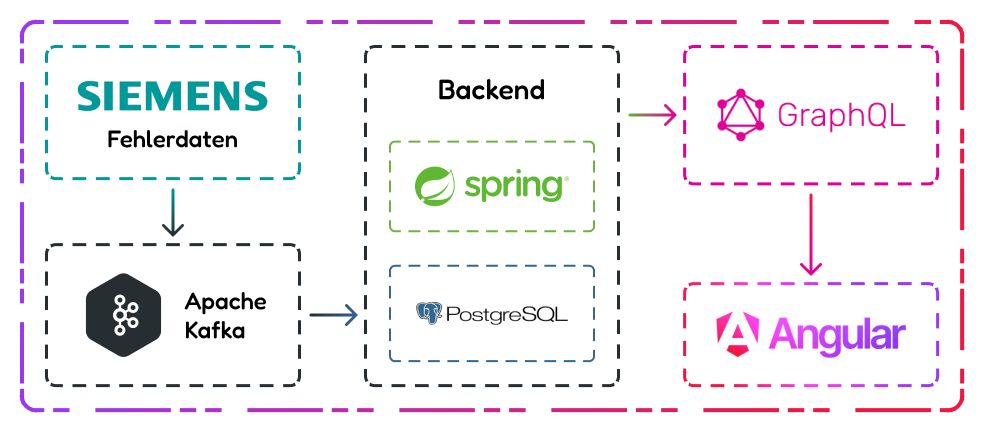
\includegraphics[width=0.8\textwidth]{content/img/Architecture/Architecture.jpg}
    \caption{Diese Darstellung zeigt den schematischen Aufbau der Applikation.}
    \label{fig:architecture_einleitung}
\end{figure}
\FloatBarrier